\documentclass{ltjsarticle}

\usepackage{amsmath}
\usepackage{amssymb}
\usepackage{amsthm}
\usepackage{ mathrsfs }
\usepackage{enumerate}
\usepackage{bbm}
\usepackage{lipsum}
\usepackage{fancyhdr}
\usepackage{tikz-cd} 
\usetikzlibrary{graphs}
\usepackage{luatexja-ruby} 
\usepackage{graphicx} 
\graphicspath{ {./images/} }

\newtheorem{theorem}{定理}[section] 
\newtheorem{proposition}{Proposition}[section] 
\newtheorem{definition}{定義}[section] 
\newtheorem{problem}{問題}
\newtheorem{postulate}{公準}[section] 
\newtheorem{lemma}{Lemma}[section] 
\newtheorem{notation}{Notation}[section] 
\newtheorem{remark}{注釈}[section] 
\newtheorem{corollary}{系}[section] 
\newtheorem{terminology}{Terminology}[section] 
\newtheorem{example}{例}[section] 
\newtheorem{step}{手順} 
\newtheorem{solution}{解答}[section] 
\newtheorem{fact}{事実}[section] 


\DeclareMathOperator{\diam}{diam}
\DeclareMathOperator{\Gal}{Gal}
\DeclareMathOperator{\rank}{rank}
\DeclareMathOperator{\Hom}{Hom}
\DeclareMathOperator{\Dom}{Dom}
\DeclareMathOperator{\Ann}{Ann}
\DeclareMathOperator{\grad}{grad}
\DeclareMathOperator{\Span}{Span}
\DeclareMathOperator{\interior}{int}
\DeclareMathOperator{\ind}{ind}
\DeclareMathOperator{\supp}{supp}
\DeclareMathOperator{\ob}{ob}
\DeclareMathOperator{\Spec}{Spec}
\DeclareMathOperator{\MaxSpec}{MaxSpec}
\DeclareMathOperator{\PreSh}{PreSh}
\DeclareMathOperator{\Sh}{Sh}
\DeclareMathOperator{\Fun}{Fun}
\DeclareMathOperator{\Ext}{Ext}
\DeclareMathOperator{\Aut}{Aut}
\DeclareMathOperator{\Ker}{Ker}
\DeclareMathOperator{\Image}{Im}
\DeclareMathOperator{\Coker}{Coker}
\DeclareMathOperator{\id}{id}
\DeclareMathOperator{\Mod}{Mod}
\DeclareMathOperator{\QCoh}{QCoh}
\DeclareMathOperator{\Coh}{Coh}
%\newcommand*{\name}[\num_arguments][default values]{{\color{#1}\Large #2}}
\newcommand*{\Z}{\mathbb{Z}}
\newcommand*{\Q}{\mathbb{Q}}
\newcommand*{\R}{\mathbb{R}}
\newcommand*{\multivar}[2]{{#1_1,\cdots,#1_{#2}}}
\newcommand*{\localization}[2]{#1_{\mathfrak{#2}}}
\newcommand*{\ringedspacemorph}[1]{(#1,#1^{\#})}
\newcommand*{\sheaf}[2]{(#1,{\mathcal{#2}}_{#1})}
\newcommand{\fib}[1]{%
  \mathbin{\mathop{\times}\limits_{#1}}%
}
\newcommand{\tens}[1]{%
  \mathbin{\mathop{\otimes}\displaylimits_{#1}}%
}
\title{授業ノート}
\author{ボン補習校高校数学}
\date{５月２日}

\begin{document}

\maketitle

\section{数学的帰納法と和}

数列$(a_n)_{n=1,2,\cdots}$について
\begin{equation*}
S_n = \underbrace{a_1+a_2+\cdots+a_n}_{\text{$1$から$n$番目の和}}
\end{equation*}

とすると新しい数列が作られます。例えば $a_n = n$なら

\begin{equation*}
S_5 = 1+2+3+4+5 = 15
\end{equation*}

$a_n = 2^{n-1}$なら
\begin{equation*}
S_4 = 1 + 2+ 4 + 8 = 15
\end{equation*}

$S_n$のことを
\begin{equation*}
\sum_{k=1}^n a_k
\end{equation*}

と言うふうに書いたりします。ここで$k$は$1$から$n$まで順番に$a_k$を足すと言う意味です。もちろん次のようにも書けます。

\begin{equation*}
\sum_{k=4}^8 k = 4+5+6+7+8 = 30
\end{equation*}

数学的帰納法を使って次のことを証明してみましょう。

\begin{equation*}
\sum_{k=1}^n k = {\frac 1 2}n(n+1)
\end{equation*}

$n=1$の時は
\begin{equation*}
1 = \sum_{k=1}^1 k = {\frac 1 2}1(1+1) = {\frac 1 2}2 = 1
\end{equation*}
よって成り立つ。$n-1$の時正しいとすると
\begin{equation*}
\sum_{k=1}^n k = \sum_{k=1}^{n-1} k+n = {\frac 1 2}(n-1)n +n = {\frac 1 2}n(n+1)
\end{equation*}
よって成り立つ。

\begin{equation*}
\sum_{k=1}^n 2^{k-1} =2^n-1
\end{equation*}

$n=1$の時は
\begin{equation*}
1 = \sum_{k=1}^1 2^{k-1} = 2^1-1 =1
\end{equation*}
よって成り立つ。$n-1$の時正しいとすると
\begin{equation*}
\sum_{k=1}^n 2^{k-1} = \sum_{k=1}^{n-1} 2^{k-1}+2^{n-1} = 2^{n-1}-1 +2^{n-1} =2\cdot2^{n-1}-1 = 2^n-1
\end{equation*}
よって成り立つ。

また$2$の代わりにどんな数$r$をおいても

\begin{equation*}
\sum_{k=1}^n r^{k-1} ={\frac {r^n-1} {r-1}}
\end{equation*}
となります。

\section{極限と和}

\begin{equation*}
\lim_{n\to\infty} \left({\frac 1 2}\right)^n = 0
\end{equation*}
になることは前の授業でやりましたが。これと上の式を組み合わせて次のことを証明してみましょう。
\begin{equation*}
1+{\frac 1 2}+{\frac 1 4}+{\frac 1 8}+\cdots+{\frac 1 {2^n}}+\cdots=\sum_{k=1}^\infty \left({\frac 1 2}\right)^{k-1} = 2
\end{equation*}

ここで
\begin{equation*}
\sum_{k=1}^\infty \left({\frac 1 2}\right)^{k-1}=\lim_{n\to\infty}\sum_{k=1}^n \left({\frac 1 2}\right)^{k-1}
\end{equation*}
です。

上の式より
\begin{equation*}
\lim_{n\to\infty}\sum_{k=1}^n \left({\frac 1 2}\right)^{k-1} = \lim_{n\to\infty}{\frac {1-\left({\frac 1 2}\right)^n} {1-{\frac 1 2}}} = {\frac 1 {1-{\frac 1 2}}}-{\frac 1{1- {\frac 1 2}}}\lim_{n\to\infty}\left({\frac 1 2}\right)^n = {\frac 1 {1-{\frac 1 2}}} = 2
\end{equation*}

これによってわかるのは、$0$より大きい数を無限の数足しても、和が無限にならない時があります。下の和
\begin{equation*}
\sum_{n=0}^\infty {\frac 1 {n!}} = {\frac 1 {0!}}+{\frac 1 {1!}} +{\frac 1 {2!}}+{\frac 1 {3!}} + {\frac 1 {4!}} +\cdots=1+1+{\frac 1 2}+{\frac 1 6}+{\frac 1 {24}}+\cdots
\end{equation*}
も同じように和が無限になりません。それだけでなく次の式が成り立ちます。
\begin{equation*}
e = \lim_{h\to\infty}\left(1+{\frac 1 h}\right)^h = \sum_{n=0}^\infty {\frac 1 {n!}}
\end{equation*}

今週来週二回使ってこのことを証明します。

\section{数学的帰納法と微分}



宿題でやった通り
\begin{equation*}
{\frac d {dx}}(1) = 0, {\frac d {dx}}(x) = 1,{\frac d {dx}}(x^2) = 2x
\end{equation*}
となりました。これを$x^n$についてどうなるか証明をしてみましょう。まずは次の式を証明します。
\begin{equation*}
{\frac d {dx}}(fg) = \left({\frac d {dx}}f\right)g+f\left({\frac d {dx}}g\right)
\end{equation*}
$x^2$の時にこれを使ってみると

\begin{equation*}
{\frac d {dx}}x = 1
\end{equation*}
なので
\begin{equation*}
{\frac d {dx}}x^2 = \left({\frac d {dx}}x\right)x+x\left({\frac d {dx}}x\right) = x+x = 2x
\end{equation*}

\begin{align*}
\lim_{h\to0}{\frac {f(x+h)g(x+h)-f(x)g(x)} {h}} &= \lim_{h\to0}{\frac {f(x+h)g(x+h)-f(x)g(x+h)+f(x)g(x+h)-f(x)g(x)} {h}},\\
& = \lim_{h\to0}g(x+h)\lim_{h\to0}{\frac {f(x+h)-f(x)} h}+f(x)\lim_{h\to0}{\frac {g(x+h)-g(x)} h},\\
& = \left({\frac d {dx}}f\right)g+f\left({\frac d {dx}}g\right).
\end{align*}



\begin{equation*}
{\frac d {dx}} x^n = nx^{n-1}
\end{equation*}

$n=1$のとき正しい、$n-1$の時正しいとすると

\begin{equation*}
{\frac d {dx}} x^n = \left({\frac d {dx}}x^{n-1}\right)x+x^{n-1}\left({\frac d {dx}}x\right) = (n-1)x^{n-2}\cdot x+x^{n-1} = nx^{n-1}
\end{equation*}

となります。次の関数を考えてみましょう。
\begin{equation*}
f(x) = \sum_{n=0}^\infty {\frac {x^n} {n!}} = 1+x+{\frac {x^2} {2!}}+{\frac {x^3} {3!}}+\cdots
\end{equation*}
ここで
\begin{equation*}
{\frac {n} {n!}} = {\frac 1 {(n-1)!}}
\end{equation*}
になることに注目すると
\begin{equation*}
{\frac d {dx}}f(x) = \sum_{n=0}^\infty {\frac {nx^{n-1}} {n!}} = 1+{\frac {2x} {2!}}+{\frac {3x^2} {3!}}+\cdots = 1+x+{\frac {x^2} {2!}}+\cdots = f(x)
\end{equation*}

$e$という数は$f(x) = e^x$とした時に
\begin{equation*}
{\frac d {dx}}f(x) = f(x)
\end{equation*}
となるような数でした。果たしてこれは偶然でしょうか。来週は
\begin{equation*}
e^x = \sum_{n=0}^\infty {\frac {x^n} {n!}}
\end{equation*}
となることを証明します。これは
\begin{equation*}
e^{i\theta} = \cos\theta+i\sin\theta
\end{equation*}
を証明するために最も重要なステップです。

\section{宿題}
\par\textbf{問題１}
三角形の合同条件を覚えていますか。次の三つの条件は同値（同じことを意味している）
\begin{enumerate}
\item また二つの三角形$\triangle ABC,\triangle EFG$は合同（対応する辺の長さが同じ）
\item $\triangle ABC,\triangle EFG$のそれぞれ二つの辺と挟んでいる頂点の角度が同じ。
\item $\triangle ABC,\triangle EFG$の二つの頂点の角度と、それに挟まれた辺の長さが同じ。
\end{enumerate}
次の条件が同値であることを示しましょう。
\begin{enumerate}
\item 三角形は二等辺三角形
\item ある頂点から向かい合う辺を半分にする線を引くと、その線は向かい合う辺と垂直。
\end{enumerate}
\begin{center}
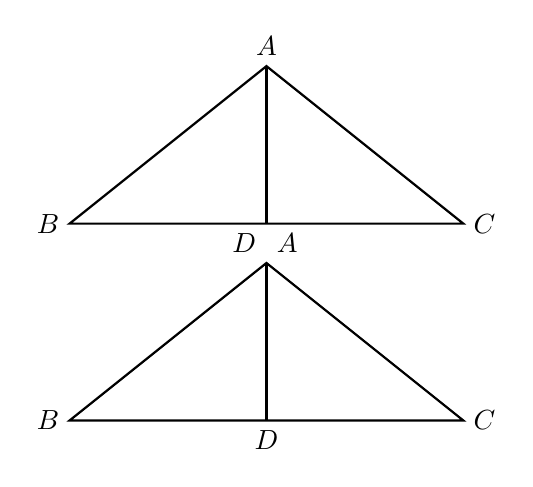
\begin{tikzpicture}
    \draw[thick] (0,0)node[left]{$B$} -- (5,0)node[right]{$C$} -- (2.5,2) node[above right]{$A$}-- cycle;
    \draw[thick] (0,2.5)node[left]{$B$} -- (5,2.5)node[right]{$C$} -- (2.5,4.5) node[above]{$A$}-- cycle;
    \draw [thick] (2.5,2) -- (2.5,0)node[below]{$D$};
    \draw [thick] (2.5,4.5) -- (2.5,2.5)node[below left]{$D$};
\end{tikzpicture}
\end{center}
\par\textbf{解答}\\
もし$\triangle ABC$が二等辺三角形なら$AB=AC$。$AD$は角$A$を半分にするので二番目の条件を使って$\triangle ADB$と$\triangle ADC$は合同。よって$\angle ADB = \angle ADC$。また$\angle ADB+\angle ADC = 180\circ$なので、$\angle ADB=\angle ADC = 90\circ$。
\par もし$AD$と$BC$が垂直なら二つの辺（$AD,DB$と$AD,DC$が同じ長さ）が同じ長さで挟まれている角$\angle ADB$と$\angle ADC$が同じなので二つの三角形$\triangle ADB$と$\triangle ADC$が合同なので$AB=AC$よって二等辺三角形。
\par\textbf{問題２オイラーグラフ（一筆書き）}
次のグラフを一筆で書きましょう。これらのグラフに共通していることはなんですか（ヒント：頂点の次数（点につながっている辺の数）を調べてみよう）
\begin{figure}[h]
	\centering
    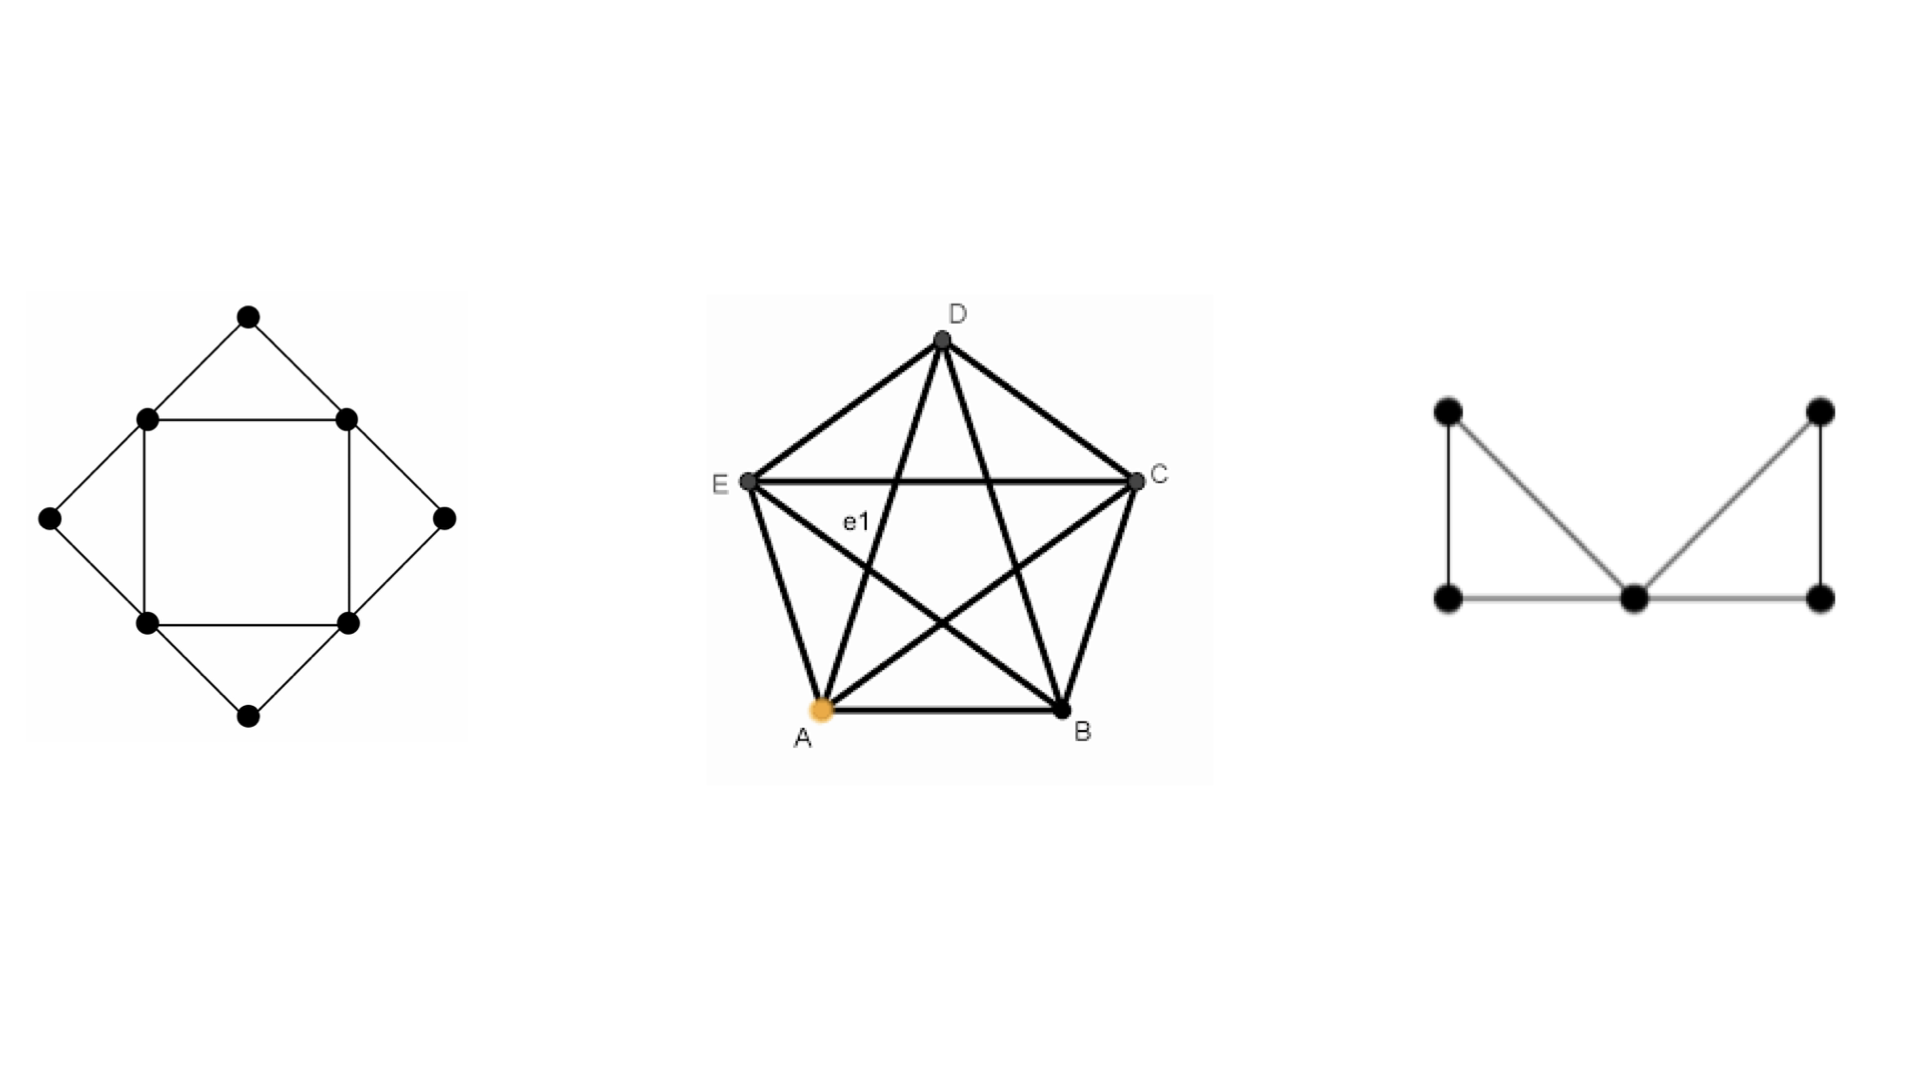
\includegraphics[scale=0.11]{euler}
    \label{fig:Euler_1}
\end{figure}
\end{document}